\chapter{Introduction}
\quad Parallel computing and software parallelization are the vast overlapping and complementary computer science areas with a history dating back to 1950s. With the advances in semiconductor industry the topics have left from high-end scientific supercomputers niche and spread to a much wider area spanning to all consumer electronic devices and are of major importance now. The parallelism is pervasive and all. Every computer scientist, software developer would benefit from having an insight into the area. Nonetheless the topics are extremely difficult and require a great deal of knowledge in various subtopics. Not all 

\section{The importance of parallel computing}
\label{parallel_computing_importance}
\quad The parallelism is pervasive and the future of computing is parallel. There are numerous factors which stress the importance of parallelism in modern computing.   

\begin{description}
\item[Abundance of natural parallelism] The field of High Performance Computing (HPC) has traditionally been concerned with scientific modelling and simulation of various natural phenomena (climate change, fluid flows, etc.). Such systems consist of numerous often independent parts. When we compile a highly parallel algorithm to a serial sequence of CPU instructions or process a huge data set with independent parts sequentially we are artificially constraining a vastly parallel computation to a serial one. Parallelism is not limited to a natural world, instead many algorithms have inherent parallelism in them.
\item[Semiconductor technology advances and power limits] With advances in transistor density it became possible to design more complicated CPUs. Initially the trend went into deeper pipelines, but running into power limits the industry design shifted towards multi core CPUs and multiprocessor systems. Such systems require of software to mirror the trend and become parallel.
\item[Domain inherent parallelism and specialized computations] The areas like computer graphics for instance have a lot of problems that can be processed in a Single Instruction Multiple Data (SIMD) fashion. That naturally led to specialized co-processors like GPUs. The hardware systems grow complex and heterogeneous.
\end{description}


\section{Challenges in Software Parallelization}
As section \ref{parallel_computing_importance} says, the parallelism in hardware has become pervasive. To achieve the full performance potential of modern hardware the software has to be mapped onto that parallel hardware. The process of software parallelization has characteristically been a very manual task, which is complex, time-consuming and error-prone.     

\subsection{Manual Parallelization Difficulties}
\quad Software parallelization has characteristically been a very manual process. As any software development process it consists of a number of stages and parts. The major problems are described below.
\begin{description}
\item[Problem understanding and partitioning] As the best software engineering practice dictates, before diving into software development one needs to thoroughly understand the problem to be solved. One needs to decide on the requirements and restrictions the final piece of software must meet. The whole algorithm and software architecture might change with the decision of developing a parallel software version instead of a serial one. If one starts from an already implemented serial software version, the parallelization might be even more difficult to do. Source code comprehension is a hard task. The algorithm chosen for a serial version might be completely unsuitable for a parallel implementation.
\item[Communications and synchronization]
\item[Implementation and data dependencies]
\item[Performance analysis and tuning] One needs to know where the program's hotspots are. Hotspots are the places where the most of the real work is being done. The majority of programs spend most of the CPU time in a few places. The task of a programmer is to find those places and concentrate all parallelization and optimization efforts right there. Finding hotspots might be difficult before the programmer has the whole program implemented. Modern hardware architectures have a multi level memory hierarchy, memory data prefetchers, TLBs, out-of-order execution, etc. It might be surprising how the actual program execution performance differs from the one inferred from the algorithm. Profilers and other analysis tools can be of help here.
\end{description}
\quad Finally, all the above challenges are interrelated and very often depend on each other. Parallel software development process can go iteratively with numerous dead ends and redesign efforts. With a long research history into the topic, all these problems are still actual now.
\subsection{Limitations of Automatic Techniques}
\quad There are various tools available to assist a programmer in the task of software parallelization. Parallelizing compilers are the most widely used.

Fully Automatic
The compiler analyzes the source code and identifies opportunities for parallelism.
The analysis includes identifying inhibitors to parallelism and possibly a cost weighting on whether or not the parallelism would actually improve performance. Loops are the most frequent target for automatic parallelization. Programmer Directed 
Using compiler directives or possibly compiler flags, the programmer explicitly tells the compiler how to parallelize the code. May be able to be used in conjunction with some degree of automatic parallelization also. The most common compiler generated parallelization is done using on-node shared memory and threads (such as OpenMP). If you are beginning with an existing serial code and have time or budget constraints, then automatic parallelization may be the answer. However, there are several important caveats that apply to automatic parallelization: Wrong results may be produced Performance may actually degrade Much less flexible than manual parallelization Limited to a subset (mostly loops) of code May actually not parallelize code if the compiler analysis suggests there are inhibitors or the code is too complex 

\begin{table}
  \begin{minipage}{\pagewidth}
  \begin{center}
    \begin{tabu}{M{3.0cm}M{1.0cm}M{3.0cm}M{1.0cm}M{3.0cm}M{1.0cm}}
      \hline
      \rowfont{\bfseries}
      reason & num & reason & num & reason & num\\\hline
      \textbf{unrecognised reduction} & 18 & \textbf{array privatization} & 7 & \textbf{AA conservativeness} & 60\\\hline
      \textbf{unknown iteration number} & 7 & \textbf{static dependencies} & 46 & \textbf{too complex} & 22\\\hline
      \textbf{uninlined calls} & 4 & \textbf{other} & 4 & \textbf{total} & 168\\\hline
    \end{tabu}
  \end{center}
  \end{minipage}
  \caption{Classification of loops missed by Intel Compiler for various reasons.}
  \label{tab:icc_missed_opportunities}
\end{table}%

We measured the running time of NASA Parallel Benchmarks after being compiled with Intel compiler (ICC) using various automatic parallelization options. Figure \ref{fig:benchmarks_runtime} illustrates the problems automatic parallelization has.

\begin{figure}[ht]
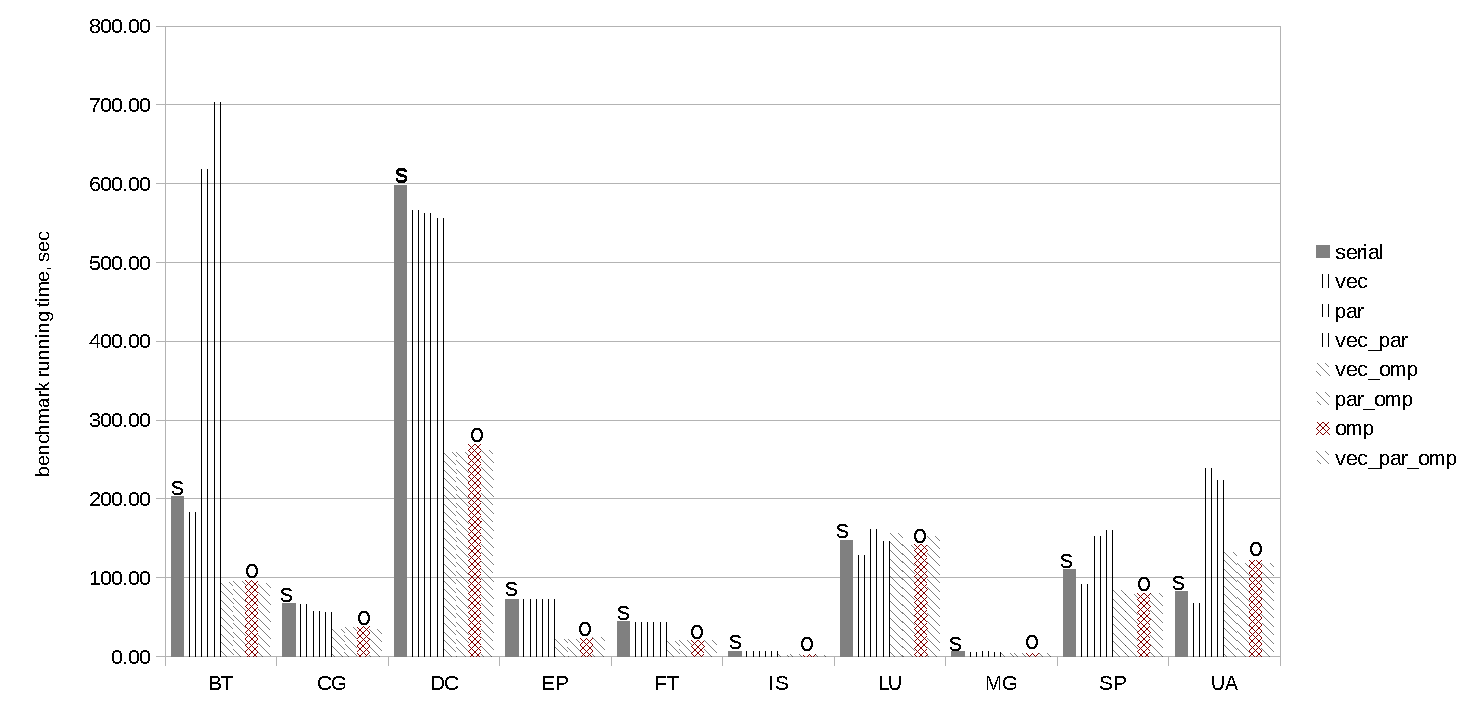
\includegraphics[width=1.0\textwidth]{images/benchmark_runtime.pdf}
\caption{The running time of various NPB benchmarks versions.}
\label{fig:benchmarks_runtime}
\end{figure}

\subsection{Limits of Machine Learning based methods}
\subsection{Data-Centric problem}
\quad As it has already been stated the problem of software parallelisation is multifaceted. There is a vast range of lower level technical issues, which can turn a perfectly parallelisable at a higher level computation into a non-parallelisable implementation. In our ML assistant project (see Chapter \ref{chapter_ml_assistant}) we showed that the main reasons of Intel Compiler failures on SNU NPB benchmarks are alias analysis conservativeness, uninlined function calls and statically unresolvable dependencies. The assistant tool we designed targets these aspects of the software parallelisation problem. But, there are many more reasons leading to non-parallelisable algorithm implementations. Source code listings \ref{lst:array} and \ref{lst:list} brightly illustrate yet another unsolved problem.\newline\null
\begin{minipage}[t]{0.45\linewidth}
\begin{lstlisting}[caption={Parallelisable loop operating on a \textbf{linear array}.},label={lst:array},language=C]
for (int i=0; i<n; it++) {
  a[i]=a[i]+1;
}
\end{lstlisting}
\end{minipage}
%
\begin{minipage}[t]{0.55\linewidth}
\begin{lstlisting}[caption={Non-parallelisable loop operating on a \textbf{linked-list}.},label={lst:list},language=C]
for (p=list; p!=NULL; p=p->next) {
  p->value+=1;
}
\end{lstlisting}
\end{minipage}
\quad Listings \ref{lst:array} and \ref{lst:list} illustrate two alternative implementations of the same simple computation. We increment all sequence elements by one. Listing \ref{lst:array} implements the sequence with a regular array linearly laid out in the memory. Listing \ref{lst:list} chooses a linked list as an implementing data structure, which leads to a source code non-parallelisability.\newline\null
\quad The DCP problem is not solved. Automatic methods are limited to relatively simple code bases such as libraries of well known data structures. The most successful methods rely on dynamic analysis and mamory graphs. Static techniques such as shape analysis are undecidable and highly conservative and might not finish in a reasonable time for the real software projects. Section [] gives a detailed literature review on the topic. 


\subsection{Parallel Programming Models}
\quad With a number of various hardware and operating system vendors entering the market with their different hardware architectures and system call interfaces software portability became a serious concern.   



To combat the problem industry vendors and major organisation came to design industry standards such as POSIX, OpenMP and MPI. 

\section{Proposed Solution}
\quad With all the problems described in the section [], we make a yet another step towards alleviating the challenging task of software parallelization. In our work we propose some ideas that might be elaborated further on. We prototype our ideas on the real benchmarks and show their potential. The first idea is that of a software parallelization assistant. The second ideas proposes a notion of computational frameworks. We ship the C++ library with the prototype implementation. The frameworks have been used to rewrite the old legacy C Olden benchmarks to a higher abstraction levels and achieve some parallel speedups.
\subsection{Software Parallelization Assistant}

\subsection{Computational Frameworks}
\quad In this work we propose an idea of computational frameworks. As algorithms and data structures are often inseparable we blend the two into the notion of a computational framework.  


